\documentclass[12pt]{article}
\usepackage[russian]{babel}
\usepackage{amsmath}
\usepackage{amssymb}
\usepackage{fontspec}
\usepackage[T1,T2A]{fontenc}
\usepackage{graphicx}
\usepackage{listings}
\setmainfont{Liberation Serif}
\oddsidemargin = -5mm
\topmargin = -20mm
\textheight = 230mm
\textwidth = 170mm
\usepackage{indentfirst}
\usepackage{xcolor}


\begin{document}

\begin{titlepage}

	\if 0
	\begin{center}
		\includegraphics[width=0.4\textwidth]{image/msu.jpg}
	\end{center}
	\fi

	\centerline{Московский государственный университет имени
	М. В. Ломоносова}
	\centerline{Факультет вычислительной математики и кибернетики}
	\centerline{Кафедра автоматизации систем вычислительных комплексов}


	\vfill
	\vfill

	\centerline{Кузьмин Ярослав Константинович}
	\centerline{}
	\large
	\bfseries
	\centerline{Разработка метода классификации сетевых пакетов}
	\centerline{с использованием графического процессорного устройства}

	\vfill

	\mdseries
	\normalsize

	\centerline{ОТЧЁТ, вариант 14}

	\vfill
	\vfill
	\vfill

	\centerline{Москва, 2022}

\end{titlepage}

\setcounter{page}{2}

\section{Постановка задачи}

Дана функция $f(x, y, z) = \sin(x^2 + z^2) y$.
Требуется написать программу с использованием технологии MPI для
вычисления значения интеграла методом Монте-Карло.

$$
I = \int\int\limits_G\int f(x, y, z) dx dy dz
$$

$$
G = \{(x, y, z) : x \geqslant 0, y \geqslant 0, z \geqslant 0, x^2 + y^2 +
z^2 \leqslant 1\}
$$

Проведём аналитическое решение данного интеграла.
Перейдём к цилиндрической системе координат:

{
	$$\left\{
	\begin{tabular}{l}
		$y = y$ \\
		$x = r \cos\phi$ \\
		$z = r \sin\phi$ \\
		$J = r$ \\
	\end{tabular}
	\right.$$
}

Интеграл принимает вид
$$
I = \int\limits_0^1 \int\limits_0^{\frac{\pi}{2}} \int\limits_0^{\sqrt{1 - y^2}}
\sin(r^2) y r dr d\phi dy =
\frac{1}{2}
\int\limits_0^1 y \int\limits_0^{\frac{\pi}{2}} \int\limits_0^{\sqrt{1 - y^2}}
\sin(r^2) d(r^2) d\phi dy =
$$
$$
= - \frac{1}{2}
\int\limits_0^1 y \int\limits_0^{\frac{\pi}{2}}
\left. \cos(r^2) \right|_0^{\sqrt{1 - y^2}} d\phi dy =
- \frac{1}{2}
\int\limits_0^1 y \int\limits_0^{\frac{\pi}{2}}
(\cos(1 - y^2) - 1) d\phi dy =
$$
$$
= \frac{1}{2}
\int\limits_0^1 y \int\limits_0^{\frac{\pi}{2}} d\phi dy -
\frac{1}{2}
\int\limits_0^1 y \int\limits_0^{\frac{\pi}{2}}
\cos(1 - y^2) d\phi dy =
\frac{\pi}{4}
\int\limits_0^1 y dy -
\frac{\pi}{4}
\int\limits_0^1 \cos(1 - y^2) y dy =
$$
$$
= \frac{\pi}{8} \left. y^2 \right|_0^1 +
\frac{\pi}{8}
\int\limits_0^1 \cos(1 - y^2) d(1 - y^2) =
\frac{\pi}{8} +
\frac{\pi}{8} \left. \sin(1 - y^2) \right|_0^1 =
$$
$$
= \frac{\pi}{8} (1 - \sin(1)) \approx 0.06225419868854213
$$

\section{Поиск приближённого решения}

Поиск значения интеграла методом Монте-Карло работает следующим образом:
рассматривается прямоугольный параллелепипед
$\Pi = \{(x, y, z) :
a_1 \leqslant x \leqslant b_1,
a_2 \leqslant y \leqslant b_2,
a_3 \leqslant z \leqslant b_3\}$ такой что
$G \subseteq \Pi$.

$$
F(x, y, z) = \begin{cases}
	f(x, y, z),& (x, y, z) \in G \\
	0,& (x, y, z) \notin G \end{cases}
$$

Случайным образом в $\Pi$ выбираются $n$ точек $p_1, \ldots, p_n$.
Приближённое значение интеграла вычисляется по формуле
$$
I \approx |\Pi|\frac{1}{n}\sum_{i=1}^n F(p_i)
$$

\section{Описание программы}

Программа использует парадигму <<мастер --- рабочие>>.
Процесс с индексом 0 генерирует точки и распределяет их для вычисления суммы
между остальными процессами с помощью функции MPI\_Scatterv.
Остальные процессы при получении своего сегмента
точек вычисляют значение $F(p)$ в них и суммируют полученые значения.
Далее происходит поиск суммы значений, полученных процессами,
с помощью операции редукции с использованием функции MPI\_Reduce.
Результат редукции получает процесс с индексом 0, который вычисляет
приближённое значение интеграла и принимает решение о продолжении вычислений
или об их остановке на основе значения интеграла, полученного аналитически и
значения $\varepsilon$. На каждой итерации генерируется 20000 точек.

\section{Результаты}

\begin{center}
	\begin{tabular}{|l|l|l|l|l|}
		\hline
		Точность $\varepsilon$ &
		Число MPI-процессов &
		Время работы программы (с) &
		Ускорение &
		Ошибка \\
		\hline
		& 2 & 0.061308 & 1 & $1.83 \cdot 10^{-5}$ \\
		\cline{2-5}
		$3.0 \cdot 10^{-5}$
		& 4 & 0.2352 & 0.260663 & $1.553 \cdot 10^{-5}$ \\
		\cline{2-5}
		& 16 & 0.196815 & 0.311501 & $4.8 \cdot 10^{-6}$ \\

		\hline
		& 2 & 0.927436 & 1 & $1.29 \cdot 10^{-6}$ \\
		\cline{2-5}
		$5.0 \cdot 10^{-6}$
		& 4 & 0.442445 & 2.096161 & $2.35 \cdot 10^{-6}$ \\
		\cline{2-5}
		& 16 & 0.664359 & 1.395986 & $3.02 \cdot 10^{-6}$ \\

		\hline
		& 2 & 1.042007 & 1 & $1.4 \cdot 10^{-6}$ \\
		\cline{2-5}
		$1.5 \cdot 10^{-6}$
		& 4 & 0.327713 & 3.179632 & $4.36 \cdot 10^{-7}$ \\
		\cline{2-5}
		& 16 & 2.791492 & 0.373279 & $4.82 \cdot 10^{-7}$ \\
		\hline
	\end{tabular}

	\medskip

	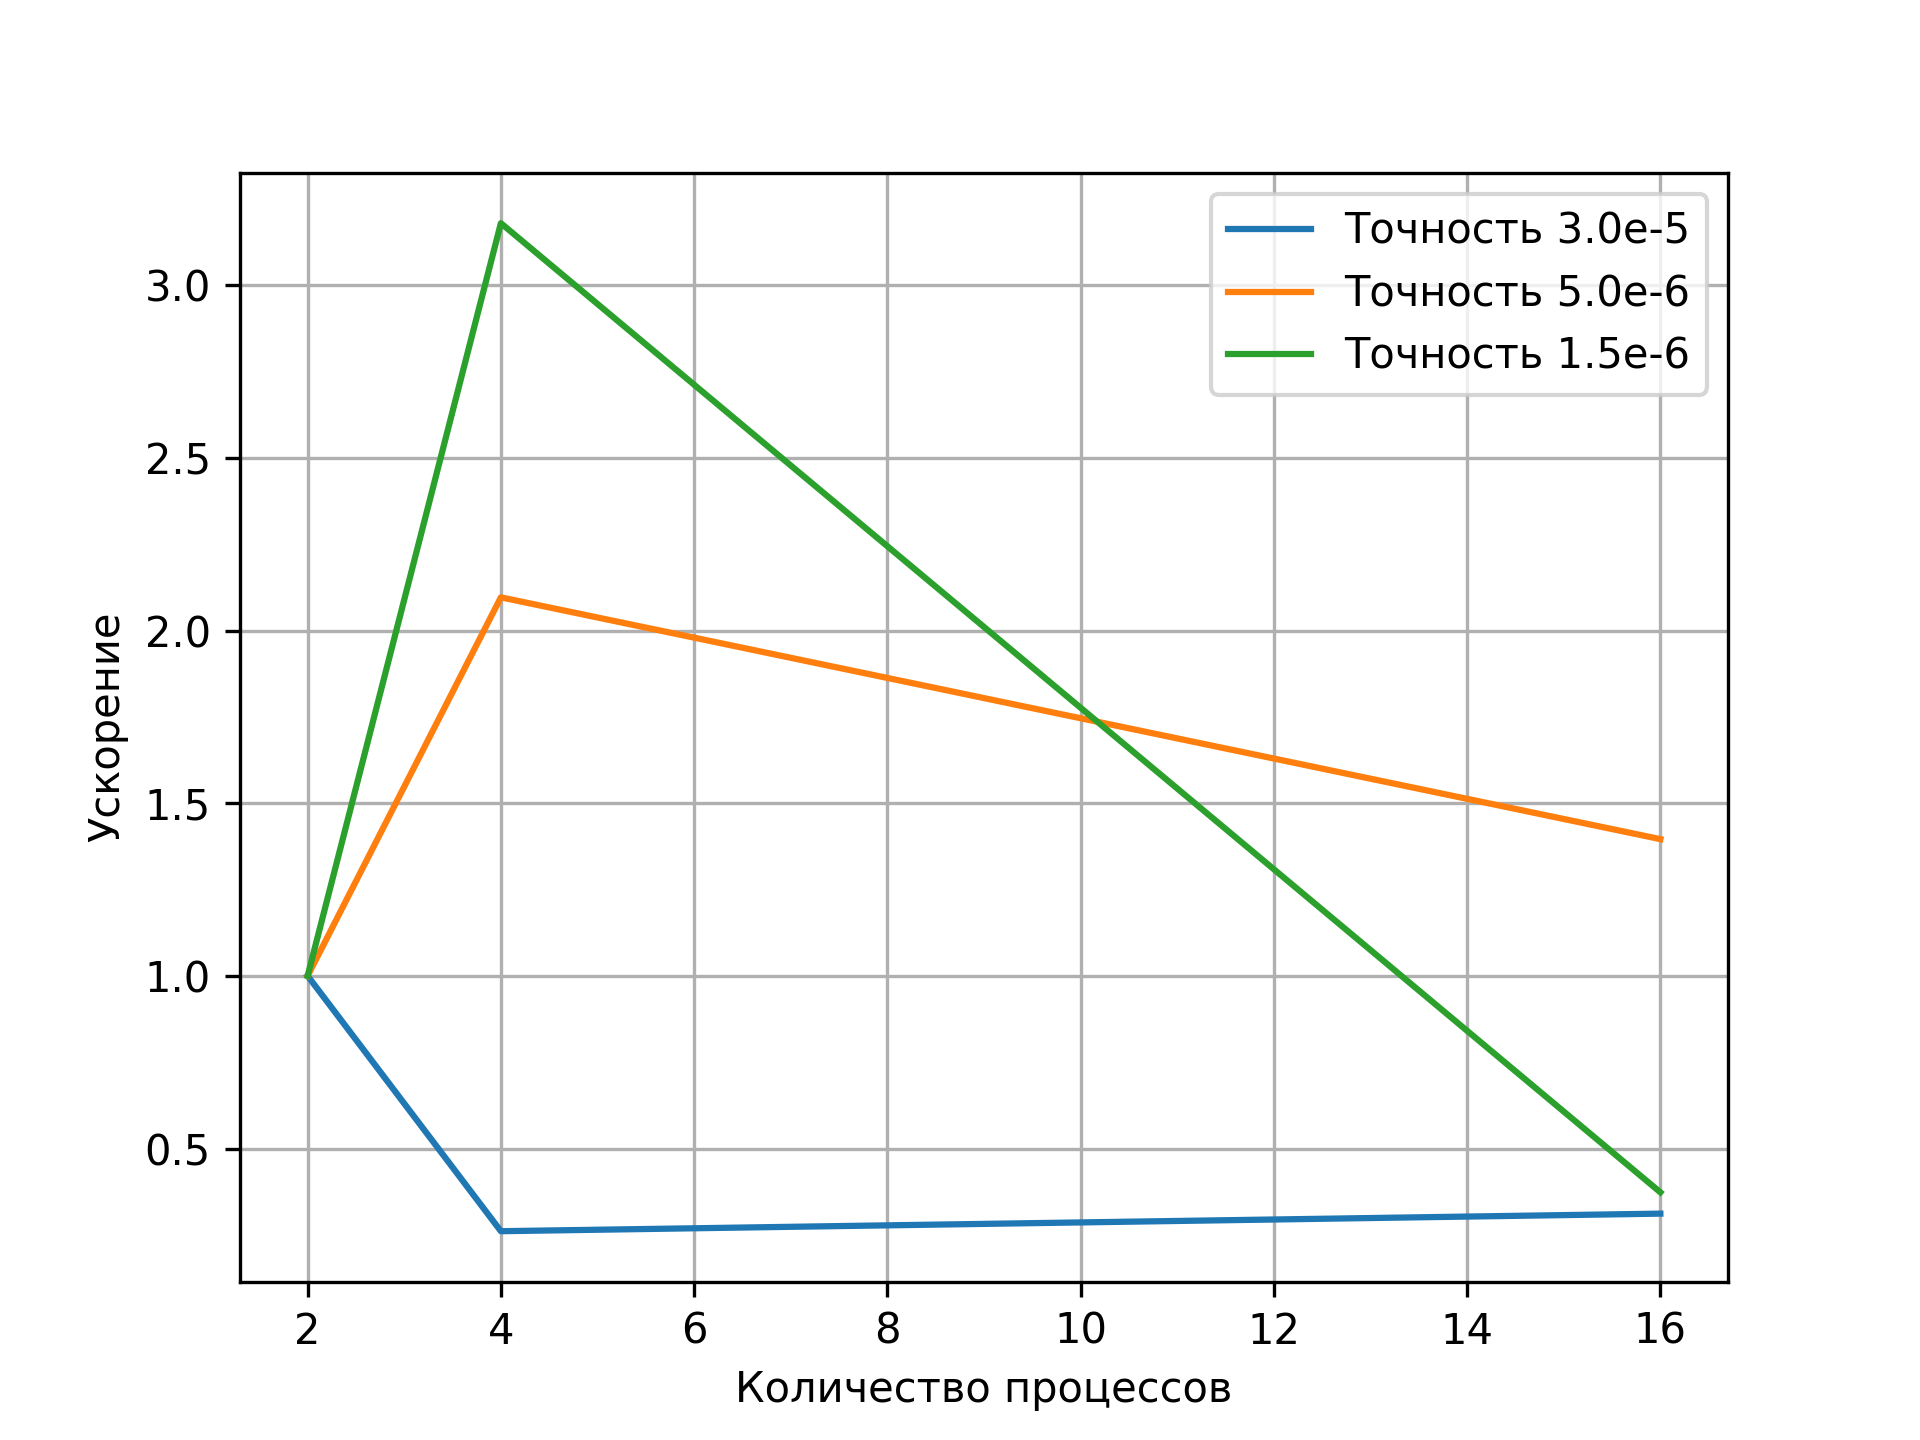
\includegraphics[width=0.9\textwidth]{plot.png}
\end{center}

\end{document}
